\scanpage{33}
\mspage{4}
\margin{32}
\[
(2'')\quad\boxed{\widetilde c_a^\omega(\lambda_{\widetilde P_a^\omega})
=\widetilde c_a^{\unsure{\omega}}(\lambda_{\widetilde P_a^{\omega'}})}
\]
en présence de $(1)$, c'est une conséquence de $(2')$, qui équivaut à la relation \unsure{déduite} de $(2')$ en le passant au carré

\diagram{\begin{tikzcd}[ampersand replacement=\&, column sep=huge]
Q \arrow[r,bend left=45,"{\mu,\unsure{\varphi}}"] \arrow[r,bend left=22,"\mu'"'] \&
Q^\vee \arrow[l,bend left=22,"\mu^\vee"'] \arrow[l,bend left=48,"\mu'{}^\vee"]
\end{tikzcd}}
\[
\underbrace{\mu^\vee\mu}_{\lambda}=\underbrace{\mu'{}^\vee\mu'}_{\lambda'}
\qquad
\underbrace{\mu'{}^{\vee-1}\mu^\vee}_{\unsure{\ }}
=\underbrace{\mu'\mu^{-1}}_{\unsure{\ }}
\quad\inserted{\searrow\ (\mu'{}^{-1}\mu)^{-1}}
\]
\[
\mu'=1,\quad\mu'{}^\vee=\mu^\vee
\quad\Longleftarrow\quad\mu^\vee=\mu'{}^\vee\mu'
\]

\hrule
\medskip
\figure{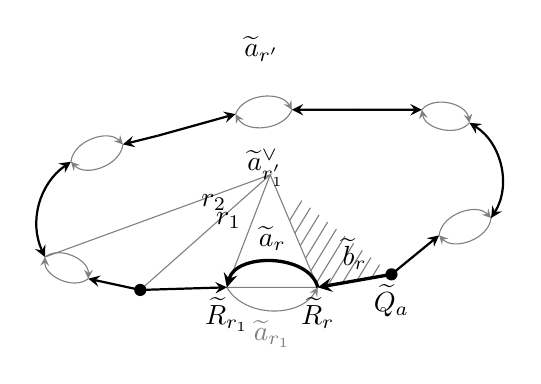
\begin{tikzpicture}[scale=1.1,>=stealth]
\coordinate (a) at (-3.0,0.4);\coordinate (b) at (-2.5,0.15);
\coordinate (c) at (-2.7,1.5);\coordinate (d) at (-2.1,1.7);
\coordinate (e) at (-0.8,2.05);\coordinate (f) at (-0.15,2.1);
\coordinate (g) at (1.35,2.1);\coordinate (h) at (1.9,1.95);
\coordinate (i) at (1.55,0.65);\coordinate (j) at (2.15,0.85);
\coordinate (k) at (-0.9,0.05);\coordinate (l) at (0.15,0.05);
\coordinate (q) at (1,0.2);\coordinate (u) at (-1.9,0.02);
\coordinate (o) at (-0.4,1.35);
\draw[gray] (a)--(o)--(u);\draw[gray] (o)--(l)--(k)--cycle;
\begin{scope}\clip (o)--(q)--(l)--cycle;
\foreach \x in {-0.8,-0.65,...,1.4}{\draw[gray] (\x,-0.2)--++(1.1,1.8);}\end{scope}
\draw[gray,->] (a) to[bend left=65] (b);\draw[gray,->] (b) to[bend left=65] (a);
\draw[gray,->] (c) to[bend left=65] (d);\draw[gray,->] (d) to[bend left=65] (c);
\draw[gray,->] (e) to[bend left=65] (f);\draw[gray,->] (f) to[bend left=65] (e);
\draw[gray,->] (g) to[bend left=65] (h);\draw[gray,->] (h) to[bend left=65] (g);
\draw[gray,->] (i) to[bend left=65] (j);\draw[gray,->] (j) to[bend left=65] (i);
\draw[very thick,->] (l) to[bend right=75] node[above] {$\widetilde a_r$} (k);
\draw[gray,->] (k) to[bend right=60] node[below] {$\widetilde a_{r_1}$} (l);
\draw[thick,<->] (a) to[bend left=40] (c);
\draw[thick,->] (-1.7,1.8)--(d);\draw[thick,->] (-1.7,1.8)--(e);
\draw[thick,->] (.6,2.1)--(f);\draw[thick,->] (.6,2.1)--(g);
\draw[thick,<->] (h) to[bend left=45] (j);
\draw[thick,->] (q)--(i);\draw[very thick,->] (q)--node[above] {$\widetilde b_r$}(l);
\draw[thick,->] (u)--(b);\draw[thick,->] (u)--(k);
\foreach \p in {u,q}{\fill (\p) circle (2pt);}
\node[below] at (k) {$\widetilde R_{r_1}$};\node[below] at (l) {$\widetilde R_r$};\node[below] at (q) {$\widetilde Q_a$};
\node[above] at (-.5,2.55) {$\widetilde a_{\unsure{r'}}$};
\node[below] at (-.45,1.75) {$\widetilde a_{\unsure{r'_1}}^{\unsure{\vee}}$};
\node at (-1.05,1.03) {$r_2$};\node at (-.88,.82) {$r_1$};
\end{tikzpicture}}

\[
\boxed{
\overbrace{\widetilde A_{\omega^n r''}\widetilde A_{\omega^{\unsure{m}}r''}\cdots\widetilde A_{r''}}^{\mu_{\widetilde Q_a}^{\omega}}
=\overbrace{\widetilde A_{\omega^n r_1}\widetilde A_{\omega^{n-1}r_1}\cdots\widetilde A_{r_1}}^{\mu_{\widetilde Q_{\unsure{i}}}^{\omega'}}}
\]
équivalent à ceci, \deleted{\unsure{bien que}}
\[
\deleted{\widetilde B'_{\omega^n r}\widetilde B_{\omega r}\cdots\widetilde B_{\unsure{r^*}}=\mu_r}
\]
\figure{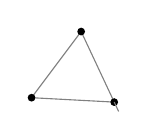
\begin{tikzpicture}[scale=.7]
\draw[gray] (0,0)--(.9,1.2)--(1.5,-.08)--cycle;
\fill (0,0) circle (2pt);\fill (.9,1.2) circle (2pt);\fill (1.5,-.08) circle (2pt);
\draw[gray] (1.5,-.08)--(1.58,-.25);
\end{tikzpicture}}
